% This file was created with tikzplotlib v0.10.1.
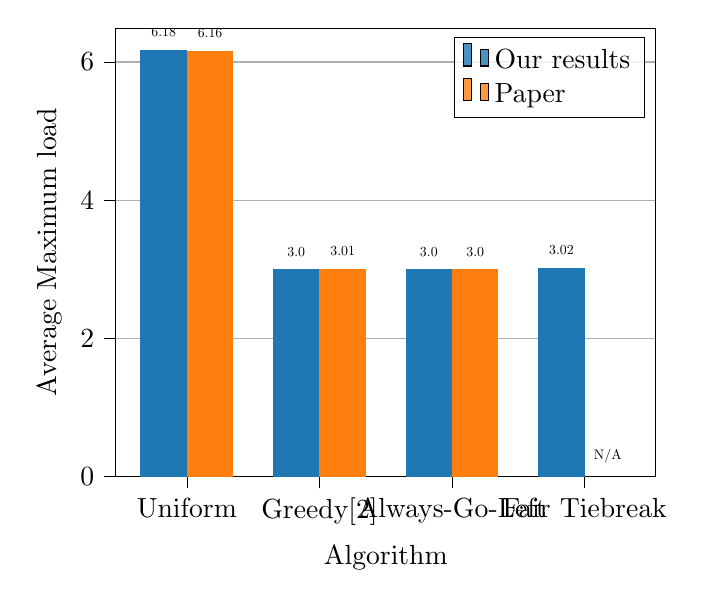
\begin{tikzpicture}

\definecolor{darkgray176}{RGB}{176,176,176}
\definecolor{darkorange25512714}{RGB}{255,127,14}
\definecolor{steelblue31119180}{RGB}{31,119,180}

\begin{axis}[
legend cell align={left},
legend style={fill opacity=0.8, draw opacity=1, text opacity=1},
tick align=outside,
tick pos=left,
x grid style={darkgray176},
xlabel={Algorithm},
xmin=-0.535, xmax=3.535,
xtick style={color=black},
xtick={0,1,2,3},
xticklabels={Uniform,Greedy[2],Always-Go-Left,Fair Tiebreak},
y grid style={darkgray176},
ylabel={Average Maximum load},
ymajorgrids,
ymin=0, ymax=6.489,
ytick style={color=black}
]
\draw[draw=none,fill=steelblue31119180] (axis cs:-0.35,0) rectangle (axis cs:0,6.18);
\addlegendimage{ybar,ybar legend,draw=none,fill=steelblue31119180}
\addlegendentry{Our results}

\draw[draw=none,fill=steelblue31119180] (axis cs:0.65,0) rectangle (axis cs:1,3);
\draw[draw=none,fill=steelblue31119180] (axis cs:1.65,0) rectangle (axis cs:2,3);
\draw[draw=none,fill=steelblue31119180] (axis cs:2.65,0) rectangle (axis cs:3,3.02);
\draw[draw=none,fill=darkorange25512714] (axis cs:2.77555756156289e-17,0) rectangle (axis cs:0.35,6.16);
\addlegendimage{ybar,ybar legend,draw=none,fill=darkorange25512714}
\addlegendentry{Paper}

\draw[draw=none,fill=darkorange25512714] (axis cs:1,0) rectangle (axis cs:1.35,3.01);
\draw[draw=none,fill=darkorange25512714] (axis cs:2,0) rectangle (axis cs:2.35,3);
\draw[draw=none,fill=darkorange25512714] (axis cs:3,0) rectangle (axis cs:3.35,0);
\draw (axis cs:-0.175,6.18) ++(0pt,3pt) node[
  scale=0.5,
  anchor=south,
  text=black,
  rotate=0.0
]{6.18};
\draw (axis cs:0.825,3) ++(0pt,3pt) node[
  scale=0.5,
  anchor=south,
  text=black,
  rotate=0.0
]{3.0};
\draw (axis cs:1.825,3) ++(0pt,3pt) node[
  scale=0.5,
  anchor=south,
  text=black,
  rotate=0.0
]{3.0};
\draw (axis cs:2.825,3.02) ++(0pt,3pt) node[
  scale=0.5,
  anchor=south,
  text=black,
  rotate=0.0
]{3.02};
\draw (axis cs:0.175,6.16) ++(0pt,3pt) node[
  scale=0.5,
  anchor=south,
  text=black,
  rotate=0.0
]{6.16};
\draw (axis cs:1.175,3.01) ++(0pt,3pt) node[
  scale=0.5,
  anchor=south,
  text=black,
  rotate=0.0
]{3.01};
\draw (axis cs:2.175,3) ++(0pt,3pt) node[
  scale=0.5,
  anchor=south,
  text=black,
  rotate=0.0
]{3.0};
\draw (axis cs:3.175,0) ++(0pt,3pt) node[
  scale=0.5,
  anchor=south,
  text=black,
  rotate=0.0
]{N/A};
\end{axis}

\end{tikzpicture}
